\documentclass{article}

% Language setting
% Replace `english' with e.g. `spanish' to change the document language
\usepackage[english]{babel}

% Set page size and margins
% Replace `letterpaper' with `a4paper' for UK/EU standard size
\usepackage[letterpaper,top=2cm,bottom=2cm,left=3cm,right=3cm,marginparwidth=1.75cm]{geometry}

% Useful packages
\usepackage{amsmath}
\usepackage{graphicx}
\usepackage[colorlinks=true, allcolors=blue]{hyperref}
\usepackage{longtable}
% \usepackage{algorithm}
\usepackage[linesnumbered,ruled,vlined]{algorithm2e}
\usepackage{algorithmic}
\usepackage{enumitem}

\usepackage{csvsimple}
\usepackage{booktabs}
\usepackage{siunitx}

% Package for code highlight and configuration code style
\usepackage{minted}
\usepackage{listings}
\usepackage[table,xcdraw]{xcolor}
\definecolor{bgcolor}{rgb}{1.0, 1.0, 0.94}
\setminted{bgcolor=bgcolor}

% Shortcut for cypher code
\newcommand{\cyphercode}[1]{
    \begin{minted}{CYPHER}
#1
    \end{minted}
}


\title{Movie Recommendation with Graph Database in Neo4j}
\author{VISWANATHAN Kartik \and DANG Ba-Khuong \and ORIANI Luca}

\begin{document}
\maketitle


\section{Introduction}

The goal of this project is to predict the rating a user might assign to a specific movie. Starting with a known user-movie pair, the system estimates a predicted rating by analyzing similar user preferences and movie attributes. The performance of the recommendation model is evaluated by comparing the actual ratings in the dataset against the predicted ratings, measuring the system's effectiveness in making accurate recommendations.

This recommendation approach, anchored in graph-based data relationships, benefits from Neo4j's capabilities in handling interconnected data structures, which can significantly enhance filtering methods. These methods analyze user-movie interactions to discover patterns and preferences that can help infer a user’s rating for a new movie.

\section{Dataset}

The $MovieLens$ dataset provides comprehensive data on user-movie interactions. There are a lot of large and complex dataset with real data as well as synthetic data. \footnote{\href{https://grouplens.org/datasets/movielens/}{https://grouplens.org/datasets/movielens/}}. In this project, we will work with a small simplified version of this dataset. Our dataset is composed of two main files: a \textbf{movies file} and a \textbf{ratings file}, each contributing essential information for our recommendation model.

\subsection{Movies File}
Movie information is contained in the file $movies.csv$. Each line of this file after the header row represents one movie, and has the following format:

\begin{minted}{BASH}
movieId,title,genres
\end{minted}

This file catalogs details of 9,125 unique movies. Each movie entry includes:

\begin{itemize}
    \item \textbf{Movie ID}: A unique identifier for each movie.
    \item \textbf{Title}: The title of the movie, often including its release year.
    \item \textbf{Genres}: The genres associated with each movie, which provide insight into the movie's content and help identify similar titles.
\end{itemize}

\subsection{Ratings File}
This file contains 100,004 user ratings, representing interactions between 671 unique users and various movies. Each rating entry includes:

\begin{minted}{BASH}
userId,movieId,rating,timestamp
\end{minted}

\begin{itemize}
    \item \textbf{User ID}: A unique identifier for each user.
    \item \textbf{Movie ID}: A reference to a movie in the movies file, linking user interactions with specific movies.
    \item \textbf{Rating}: A score given by the user to a movie, ranging from 0.5 to 5.0 in 0.5 increments.
    \item \textbf{Timestamp}: The date and time of the rating, recorded as a UNIX timestamp, which can provide temporal insights into user behavior.
\end{itemize}

The ratings scale ranges from 0.5 to 5.0, providing nuanced feedback on movies. This range allows for more granular user preferences, which is beneficial for building a refined recommendation model.

\subsection{Get to know the data}

We can perform some basic queries to understand our dataset better: 

\begin{itemize}
    \item Number of movies
    \begin{minted}{CYPHER}
    MATCH (u:User)
    RETURN COUNT(*)
    >>COUNT(*)
    >>671
    \end{minted}

    \item Number of movies
    \begin{minted}{CYPHER}
    MATCH (m:Movie)
    RETURN COUNT(*)
    >>COUNT(*)
    >>9125
    \end{minted}

    \item Users and their corresponding ratings
    \begin{minted}{CYPHER}
    MATCH (u:User)-[r:RATED]->(m:Movie)
    RETURN u.id AS user, count(*) AS nb_rating
    ORDER BY nb_rating DESC
    LIMIT 5
    
    UNION 
    
    MATCH (u:User)-[r:RATED]->(m:Movie)
    RETURN u.id AS user, count(*) AS nb_rating
    ORDER BY nb_rating
    LIMIT 5
    \end{minted}

    \autoref{tab:top5bot5rating} shows the top 5 users and bottom 5 users with the most and least number of ratings respectively. 
         
    \begin{table}[!ht]
    \centering
    \caption{Top 5 and Bottom 5 users with the most ratings}
    \label{tab:top5bot5rating}
    \begin{tabular}{lr}
    \hline
        user & nb\_rating \\ \hline
        547 & 2391 \\ 
        564 & 1868 \\ 
        624 & 1735 \\ 
        15 & 1700 \\ 
        73 & 1610 \\ 
        35 & 20 \\ 
        76 & 20 \\ 
        14 & 20 \\ 
        1 & 20 \\ 
        209 & 20 \\ \hline
    \end{tabular}
    \end{table}

    \item Movies and their corresponding genres
    \begin{minted}{CYPHER}
        MATCH (m:Movie)-[g:HAS_GENRE]->(gen:Genre)
        RETURN m.title AS movie, COUNT(*) AS nb_genres
        ORDER BY nb_genres DESC
        LIMIT 5
    \end{minted}

    \autoref{tab:top5moviehasgenres} shows the top 5 movies with the most number of genres. 
    
    \begin{table}[!ht]
    \centering
    \caption{Top 5 movies with most genres}
    \label{tab:top5moviehasgenres}
    \begin{tabular}{lr}
    \hline
        movie & nb\_genres \\ \hline
        Rubber (2010) & 10 \\ 
        Patlabor: The Movie (Kidô keisatsu patorebâ: The Movie) (1989) & 8 \\ 
        Motorama (1991) & 8 \\ 
        Wonderful World of the Brothers Grimm, The (1962) & 8 \\ 
        Mulan (1998) & 7 \\ \hline
    \end{tabular}
    \end{table}

    \item Distribution of movies and ratings. 

    We can query top 5 highest-rate and bottom 5 lowest-rate movies, which gets more than 10 ratings (to avoid bias)

    \begin{minted}{CYPHER}
    MATCH (m:Movie)<-[r:RATED]-(u:User)
    WITH m.title AS movie, AVG(r.rating) AS avg_rate, COUNT(*) AS nb_rating
    WHERE nb_rating > 10
    RETURN movie, avg_rate, nb_rating
    ORDER BY avg_rate DESC
    LIMIT 5
    
    UNION
    
    MATCH (m:Movie)<-[r:RATED]-(u:User)
    WITH m.title AS movie, AVG(r.rating) AS avg_rate, COUNT(*) AS nb_rating
    WHERE nb_rating > 10
    RETURN movie, avg_rate, nb_rating
    ORDER BY avg_rate
    LIMIT 5 
    \end{minted}

    Similarly, we can query top 5 highest-rated genres and bottom 5 lowest-rated movies. 

    \begin{minted}{CYPHER}
    MATCH (genre:Genre)<-[g:HAS_GENRE]-(m:Movie)<-[r:RATED]-(u:User)
    WITH genre.name AS genre, AVG(r.rating) AS avg_rate
    RETURN genre, avg_rate
    ORDER BY avg_rate DESC
    LIMIT 5
    
    UNION 
    
    MATCH (genre:Genre)<-[g:HAS_GENRE]-(m:Movie)<-[r:RATED]-(u:User)
    WITH genre.name AS genre, AVG(r.rating) AS avg_rate
    RETURN genre, avg_rate
    ORDER BY avg_rate 
    LIMIT 5
    \end{minted}

    \autoref{tab:top5bot5ratemovies} shows the top 5 highest-rated movies and bottom 5 lowest-rated movies. And \autoref{tab:top5bot5rategenres} shows the top 5 highest-rated genres and bottom 5 lowest-rated movies. Interestingly, we notice that there is not a big difference of average rating between the highest and the lowest. The distribution of genre's rating is very uniform.  

    \begin{table}[!ht]
    \centering
    \sisetup{table-format = 1.3} 
    \caption{Top 5 highest-rate and bottom 5 lowest-rate movies}
    \label{tab:top5bot5ratemovies}
    \begin{tabular}{@{}lS[table-auto-round]r@{}}
    \hline
        {movie} & {avg\_rate} & {nb\_rating} \\ 
        \hline
        Best Years of Our Lives, The (1946) & 4.636363636363636 & 11 \\ 
        Inherit the Wind (1960) & 4.541666666666667 & 12 \\ 
        Godfather, The (1972) & 4.487499999999999 & 200 \\ 
        Shawshank Redemption, The (1994) & 4.487138263665592 & 311 \\ 
        Tom Jones (1963) & 4.458333333333333 & 12 \\ \hline
        Battlefield Earth (2000) & 1.2105263157894737 & 19 \\ 
        Speed 2: Cruise Control (1997) & 1.6521739130434783 & 23 \\ 
        Police Academy 6: City Under Siege (1989) & 1.7083333333333335 & 12 \\ 
        Super Mario Bros. (1993) & 1.7352941176470587 & 17 \\ 
        Blade: Trinity (2004) & 1.7916666666666663 & 12 \\ \hline
    \end{tabular}
    \end{table}

    \begin{table}[!ht]
    \centering
    \sisetup{table-format = 1.3} 
    \caption{Top 5 highest-rate and bottom 5 lowest-rate movies}
    \begin{tabular}{lS[table-auto-round]}
    \hline
        {genre} & {avg\_rate} \\ \hline
        FILM-NOIR & 3.955701754385961 \\ 
        WAR & 3.817213930348258 \\ 
        DOCUMENTARY & 3.8132992327365693 \\ 
        (NO GENRES LISTED) & 3.7777777777777786 \\ 
        DRAMA & 3.681779585269913 \\ \hline
        HORROR & 3.3152430044182726 \\ 
        ACTION & 3.445612803075102 \\ 
        COMEDY & 3.44603692210594 \\ 
        SCI-FI & 3.460429547673291 \\ 
        CHILDREN & 3.4661866359446964 \\ \hline
    \end{tabular}
    \label{tab:top5bot5rategenres}
    \end{table}
    
\end{itemize}

\section{Recommendation Engine}

There are two popular methods for recommendation engine: \textbf{content-based filtering }and\textbf{ collective filtering}. In this report, we will implement both methods and compare their performance as well as their resulting metrics. The main difference between two methods is how we analyze the input feature: content-based analyzes \textit{the features of the targeted movie}, while collective-filtering analyzes the \textit{features of targeted user. }

\subsection{Content-based} \label{sec:content-base}

\textit{The Basic idea}: If someone likes something, they’ll like something similar to it as well.

The idea of content-based method is predicting score for targeted movie by analyzing the features of the movie itself. In this method, we focus on the attributes of the movie rather than behavior of collection of users.  We predict the targeted score based on the scores of similar movies that the target user has already rated. 

Our algorithm have important metrics/parameters, which we discuss below: 

\begin{itemize}
    \item Similarity score between movies: In our dataset, each movie only has 1 important attribute, which is its genre. Thus, we will define the similarity between 2 movies as how many shared genres they have.

    \item k-Nearest neighbor: the number of similar movies that we want to include in our prediction. The number of kNN \textit{k} will affect the performance of our model: small \textit{k} will make our model more flexible but it will increase risk of overfitting, and the model will be more sensitive to noise in dataset. On the other hand, large \textit{k} will make the model more robust, but it can underfit. Also, with large \textit{k} we have more computational complexity. In classical machine learning, we normally use cross-validation to fine-tune our hyperparameter, but Neo4j is not very suitable for that so we will try different value of k. 

    \item Function to predict rating: from a collection of similar movies with their rating, we will predict score for targeted movie using different function: \texttt{mean()}, \texttt{median()} and \texttt{mode()}. 
\end{itemize}

Our algorithm: 

\begin{algorithm}[H]
\caption{Content-based filtering}
\KwIn{Input targeted user $u$, targeted movie $m$}
\KwOut{Output: predicted score $predict\_score$}
Initialize 100 targeted users $u$ and corresponding tarted movies $m$\;
\For{each $u$, $m$ in the list}{
    Find other movies $m2$ that $u$ rated ($u$)-[$r2$]-($m2$)\;
    Find the number of shared genres between $m2$ and $m$ \;
    Order by number of $shared genres$ \;
    Take the first $k$ kNN $m2$ \;
    Collect $r2.rating$ \;
    Calculate predict score using: \;
        $predict\_score$ = mean($r2.rating$) or \;
        $predict\_score$ = median($r2.rating$) or \;
        $predict\_score$ = mode($r2.rating$) or \;
    }
\Return $predict\_score$\;
\end{algorithm}
\vspace{1mm}
\textbf{Neo4j implementation}

Here we demonstrate the content-based filtering method with 1 user as an example. 

We start with initial query to get targeted user (here we take user with \texttt{u.id = 10}) and targeted movie 

\begin{minted}{CYPHER}
MATCH (u:User)-[r:RATED]->(m:Movie)
WHERE u.id = 10
WITH u, collect(r) AS rcol
WITH u, head(rcol) AS r1
MATCH (u)-[r1]->(m)
WITH u, m, r1.rating AS actual_rating
\end{minted}

Next, we find other movies $m2$ that $u$ has already rated (that is not targeted movie $m$). After that, we find the common genres between $m$ and $m2$

\begin{minted}{CYPHER}
MATCH (u)-[r2:RATED]->(m2:Movie)
WHERE m2.id <> m.id
WITH u, m, actual_rating, m2, r2.rating AS r2_rating
// Find the common genres between target movie m and other movies m2
MATCH (m)-[:HAS_GENRE]->(g:Genre)<-[:HAS_GENRE]-(m2)
WITH u, m, actual_rating, 
    m2, r2_rating, 
    COLLECT(g.name) AS genres, COUNT(*) AS shared_genres
ORDER BY shared_genres DESC
\end{minted}

\autoref{tab:top10similarmovie} shows the top 10 movies that have the most number of shared genres with targeted movie. The $r2.rating$ column contains the actual rating of targeted user for each movie, which we will collect and base our prediction on. 

\begin{table}[!ht]
    \centering
    \caption{Top 10 movies that have most shared genres with targeted movie}
    \resizebox{\textwidth}{!}{%
        \begin{tabular}{llrrrrr}
            user & m & actual rating & m2 & r2 rating & genres & shared genres \\ \hline
            10 & Romancing the Stone (1984) & 4.0 & 1197 & 4.0 & [COMEDY, ADVENTURE, ROMANCE, ACTION] & 4 \\ 
            10 & Romancing the Stone (1984) & 4.0 & 2890 & 4.0 & [COMEDY, ADVENTURE, ACTION] & 3 \\ 
            10 & Romancing the Stone (1984) & 4.0 & 1101 & 2.0 & [ROMANCE, ACTION] & 2 \\ 
            10 & Romancing the Stone (1984) & 4.0 & 2826 & 5.0 & [ADVENTURE, ACTION] & 2 \\ 
            10 & Romancing the Stone (1984) & 4.0 & 1196 & 4.0 & [ADVENTURE, ACTION] & 2 \\ 
            10 & Romancing the Stone (1984) & 4.0 & 1291 & 4.0 & [ADVENTURE, ACTION] & 2 \\ 
            10 & Romancing the Stone (1984) & 4.0 & 2344 & 5.0 & [ADVENTURE, ACTION] & 2 \\ 
            10 & Romancing the Stone (1984) & 4.0 & 1198 & 4.0 & [ADVENTURE, ACTION] & 2 \\ 
            10 & Romancing the Stone (1984) & 4.0 & 2108 & 3.0 & [COMEDY, ROMANCE] & 2 \\ 
            10 & Romancing the Stone (1984) & 4.0 & 1887 & 2.0 & [COMEDY, ADVENTURE] & 2 \\ 
        \end{tabular}%
    }
    \label{tab:top10similarmovie}
\end{table}


As we mentioned earlier, we will use 3 difference functions to predict the score: \texttt{mean()}, \texttt{median()} and \texttt{mode()}. The result is shown in \autoref{tab:examplecontentbase}

\begin{table}[!ht]
    \raggedleft
    \caption{Predict rating for targeted movie}
    \begin{tabular}{rrrrrr}
        func & user & movie & actual\_rating & predict\_rating & square\_error \\ \hline
        average & 10 & Romancing the Stone (1984) & 4.0 & 3.0 & 1.0 \\ 
        mode & 10 & Romancing the Stone (1984) & 4.0 & 4.0 & 0.0 \\ 
        median & 10 & Romancing the Stone (1984) & 4.0 & 3.5 & 0.25 \\ 
    \end{tabular}
    \label{tab:examplecontentbase}
\end{table}

\subsection{Collective filtering}

\textit{The Basic idea}: If $user 1$ and $user 2$ have similar taste in movies, they’ll have similar rating for a particular movie. 

In collective filtering method, we focus on the behavior of other users that have similar taste with targeted user instead of the attributes of the movie itself.  We predict the targeted rating based on the ratings of similar users for the same targeted movie.  

Similar to content-based method, we will also use the k-Nearest neighbor hyperparameter in our method to only select top $k$ users that have largest similarity score with targeted user. Additionally, we will have more variants, which we present below. 

\begin{enumerate}[label=\alph*.]  
    \item Similarity score between users: Unlike similarity metric between movies, we will use cosine similarity as our metric to measure similarity score between 2 users. 
    
    Cosine similarity is the cosine of the angle between two n-dimensional vectors in an n-dimensional space. Mathematically, it is the dot product of the two vectors divided by the product of the two vectors' lengths.

    In our context, cosine similarity of $user 1$ and $user 2$  will be based on vector of ratings of common movies between them. For example, \(u_1\) has rating vector \(r_1 = \begin{matrix}[3 & 4 & 4 & 5]\end{matrix}^T\) and \(u_2\) has rating vector \(r_2 = \begin{matrix}[2 & 3 & 2 & 4]\end{matrix}^T\)
    
    \[
    \text{cosine\_similarity}(u_1, u_2) = cos(\theta) = \frac{r_1 \cdot r_2}{\|r_1\| \|r_2\|}
    \]

    Notice that in a vector space \(R^n\), \(cos(\theta)\) ranges from \([-1, 1]\) with negative indicated 2 users have opposite preference. But in our dataset, we have non-negative rating, which means \(r_1\) and \(r_2\) will always be positive. Thus, we will always have positive similarity score. 
    
    Here, we present the first variation of our algorithm: we will use 2 different methods in calculating cosine similarity: \textbf{normalized similarity} and \textbf{non-normalized similarity}.

    \begin{itemize}
        \item \textit{Non-normalized similarity} will be calculated as shown above.

        \item \textit{Normalized similarity}: we normalize the rating vector for each user before wrap them in the cosine function. The new rating vector will be: 
        \[
        \tilde{r} = 
        \begin{pmatrix}
            r_1 - \bar{r} \\
            r_2 - \bar{r} \\
            \vdots \\
            r_n - \bar{r}
        \end{pmatrix} \\
        \text{with } \bar{r} = n^{-1} \sum_{i=1}^{n}{r_i}
        \]
    \end{itemize}

    \item Here is our second variation of the method: predict rating by averaging technique and by binning technique. We will present the averaging technique in section \ref{sec:similarityscore}, and the binning technique will be discussed in section \ref{sec:bintechnique}
    
\end{enumerate}

Our algorithm for collective filtering is summarized as follow: 

\begin{algorithm}[H]
\caption{Collective Filtering}
\KwIn{Input targeted user $u$, targeted movie $m$}
\KwOut{Output: predicted score $predict\_score$}
Initialize 100 targeted users $u$ and corresponding tarted movies $m$\;
\For{each $u$, $m$ in the list}{
    Find list of other users $list(u2)$ that rated the targeted movie ($u2$)-[$r2$]-($m$)\;
    \For{each $u2$ in the list}{
        Find other $common_movies$ that $u$ and $u2$ rate in common \;
        Collect rating vector $r1.rating$ and $r2.rating$ \;
        Calculate cosine similarity between $u$ and $u2$ \;
        Create and write similarity relationship \; 
    }
    Order by $similarity score$ \;
    Take the first $k$ kNN $u2$ \;
    Collect $r2.rating$ \;
    Calculate $predict score$ using: avg or binning technique
    }
\Return $predict\_score$\;
\end{algorithm}


\subsubsection{Collective filtering with similarity score }\label{sec:similarityscore}

We will demonstrate collective filtering using the same example $user.id = 10$ as section \ref{sec:content-base}.

First, we find other users that also rate the targeted movie: 

\begin{minted}{CYPHER}
MATCH (u2:User)-[r2:RATED]->(m)
WHERE u2.id <> u.id  // Exclude user 1
WITH u, m, actual_rating, u2, r2.rating AS r2

RETURN u, m, actual_rating, u2, r2
\end{minted}

\begin{figure}[htbp]
    \centering
    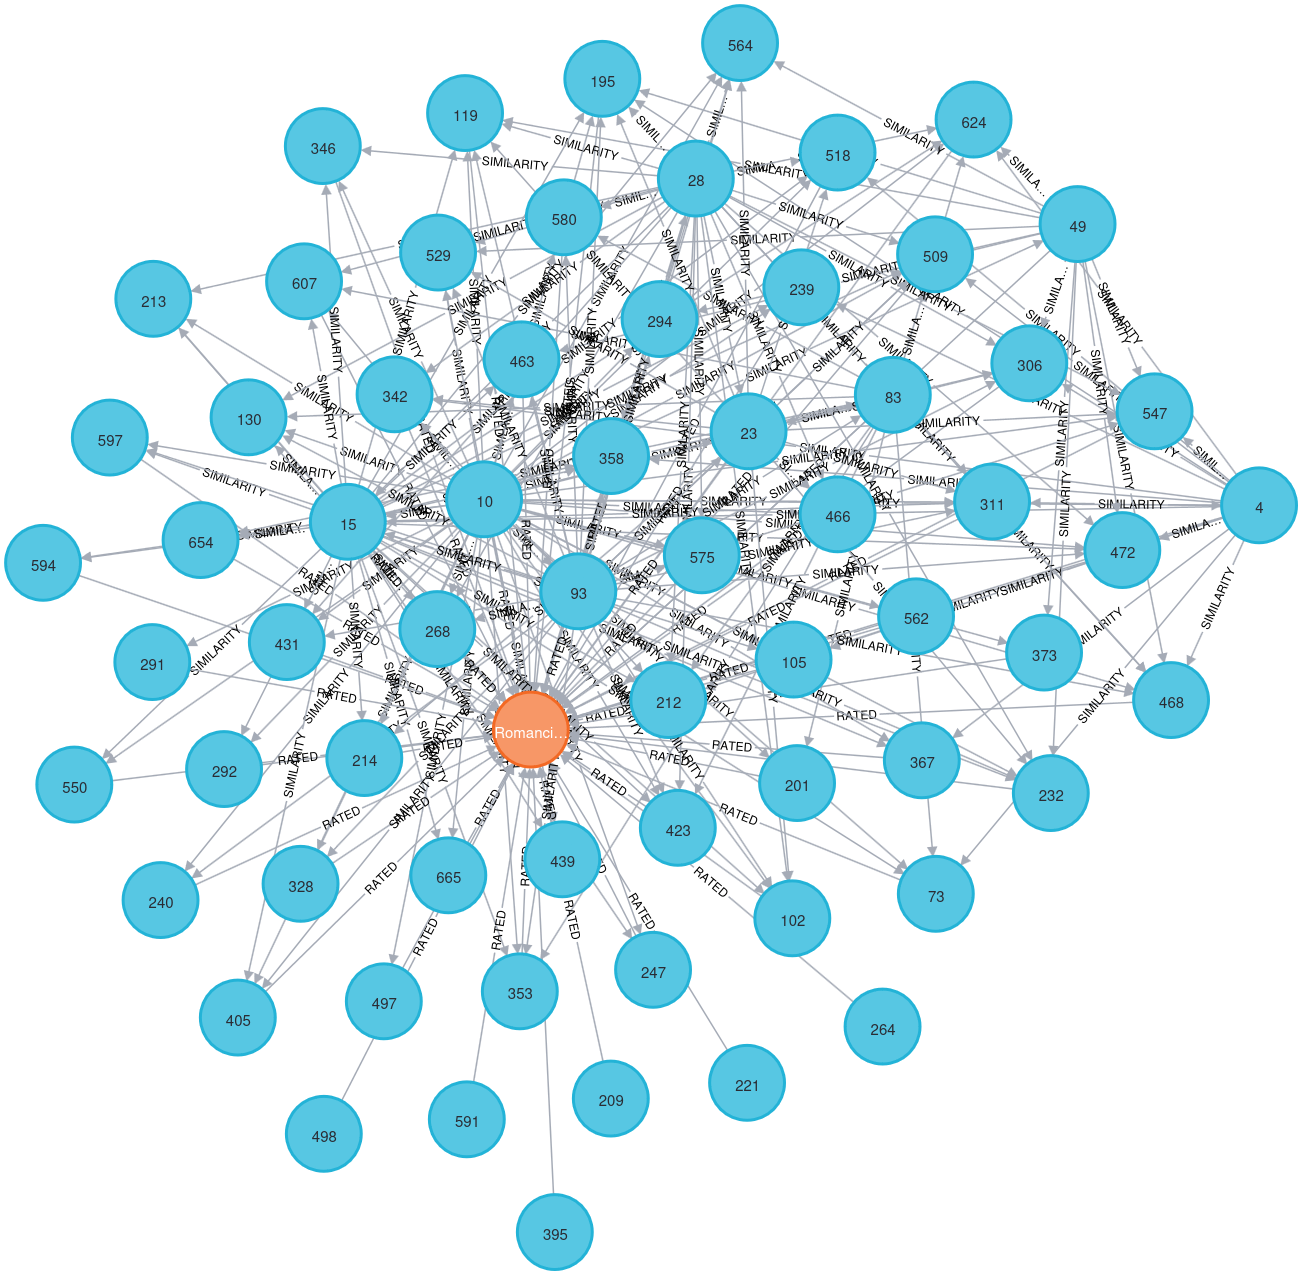
\includegraphics[width=0.7\textwidth]{figures/graph-u2-rate-m.png} 
    \caption{Other users who also rate targeted movie}
    \label{fig:graph-u2-rate-m}
\end{figure}

\autoref{fig:graph-u2-rate-m} show the graph display of other users who also rate the targeted movie. In particular, we have 64 other users (excluding target user $id=10$). Next, we will find other common movies (excluding targeted movie) between $u$ and each $u2$. 

\begin{minted}{CYPHER}
MATCH (u)-[r1_common:RATED]->(common_movie:Movie)<-[r2_common:RATED]-(u2)
WHERE common_movie.id <> m.id

WITH u, m, actual_rating, u2, r2,
    COUNT(common_movie) AS nb_common_movie, 
    COLLECT(r1_common.rating) AS u_common_ratings,
    COLLECT(r2_common.rating) AS u2_common_ratings
WHERE nb_common_movie > 3
ORDER BY nb_common_movie DESC
\end{minted}

Here we apply another constrain to our query: we only return user that has more than 3 common movies with $u$. The reason for this constrain is to stabilize our model so it will work even we do not normalize the rating vector. 

For example: if we have \(u_1 \text{and} u_2\) only share 1 common movie, with rating 2 and 5 respectively. We can see that they have opposite preference for this movie, but mathematically their cosine similarity will be 1, which indicate perfect match. In general, cosine function for vector in \(R^1\) will guarantee be 1, which is obviously not true.   

\[
\text{cosine\_similarity}(u_1, u_2) =  \frac{2 \cdot 5}{\|2\| \|5\|} = 1
\]

Now we have the rating vectors for common movies (of the same length) for 2 users, we can calculate similarity score between them. We will create new $SIMILARITY$ relationship in our database to store this information. With similarity score, we can easily see k-nearest neighbor of any targeted user. \autoref{tab:top5similaruser} reports the 5 nearest neighbor of user $id = 10$ with non-normalized similarity score, and \autoref{tab:top5similarusernormalize} reports the normalized version. We notice that the value in normalized version is smaller than the normalized one, so by normalizing rating, we avoid some extreme value of similarity score (larger than 0.95). \autoref{fig:graph-5knn-similar-user} shows the graph view of \autoref{tab:top5similarusernormalize}. 


\begin{table}[H]
    \centering
    \sisetup{table-format = 1.3, table-number-alignment = right}
    \caption{Top 5 similar user of user id=10 (non-normalized)} 
    \label{tab:top5similaruser} 
    \begin{tabular}{llrrrS[table-auto-round]r}
    \hline
        u.id & m.title & actual\_rating & u2.id & r2 & similarity & nb\_common\_movie \\ \hline
        10 & Romancing the Stone (1984) & 4.0 & 4 & 5.0 & 0.9929369333777895 & 11 \\ 
        10 & Romancing the Stone (1984) & 4.0 & 328 & 3.5 & 0.9925232596048371 & 6 \\ 
        10 & Romancing the Stone (1984) & 4.0 & 550 & 4.0 & 0.9906109446539152 & 13 \\ 
        10 & Romancing the Stone (1984) & 4.0 & 291 & 4.0 & 0.9895373906723676 & 9 \\ 
        10 & Romancing the Stone (1984) & 4.0 & 93 & 3.5 & 0.9866477001496159 & 7 \\ \hline
    \end{tabular}
\end{table}


\begin{table}[H]
    \centering
    \sisetup{table-format = 1.3, table-number-alignment = right}
    \caption{Top 5 similar user of user id=10 (normalized)} 
    \label{tab:top5similarusernormalize} 
    \begin{tabular}{llrrrS[table-auto-round]r}
    \hline
        u.id & m.title & actual\_rating & u2.id & r2 & similarity & nb\_common\_movie \\ \hline
        10 & Romancing the Stone (1984) & 4.0 & 550 & 4.0 & 0.8047382152330894 & 13 \\ 
        10 & Romancing the Stone (1984) & 4.0 & 49 & 4.0 & 0.8010216453679182 & 7 \\ 
        10 & Romancing the Stone (1984) & 4.0 & 328 & 3.5 & 0.6792310117428241 & 6 \\ 
        10 & Romancing the Stone (1984) & 4.0 & 358 & 4.0 & 0.5899370655917284 & 16 \\ 
        10 & Romancing the Stone (1984) & 4.0 & 195 & 1.0 & 0.5331302814678663 & 17 \\ \hline
    \end{tabular}
\end{table}

\begin{figure}[htbp]
    \centering
    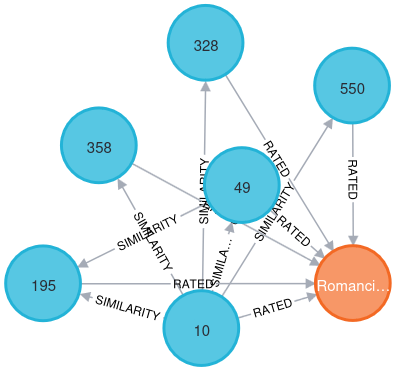
\includegraphics[width=0.7\textwidth]{figures/graph-5knn-similar-user.png} 
    \caption{Top 5 similar users who also rate targeted movie}
    \label{fig:graph-5knn-similar-user}
\end{figure}

Now we have collected everything we need to predict the rating. In this section, we will use the weighted average value of ratings: 

\[
\text{predict rating} = \frac{\sum(w_i r_{2i})}{\sum{w_i}} \\
\text{ with}: w_i: \text{similarity score of user i, and } r_{2i}: \text{rating of user i}
\]


\begin{table}[H]
    \centering
    \caption{Example result of predict rating for user id 10} 
    \label{tab:eg_collect_filter_result} 
    \begin{tabular}{lllrrr}
    \hline
        type & user & movie & actual\_rating & predict\_rating & square\_error \\ \hline
        normalize & 10 & Romancing the Stone (1984) & 4.0 & 3.5 & 0.25 \\ 
        non-normalize & 10 & Romancing the Stone (1984) & 4.0 & 4.0 & 0.0 \\ \hline
    \end{tabular}
\end{table}

\autoref{tab:eg_collect_filter_result} shows the result for our demo for 1 user: in this case, the non-normalized version performs better than the normalized one, but this will not always the case as we will see later when we run our model with big datasize. 

\subsubsection{Collective filtering with binning technique.}\label{sec:bintechnique}

The idea of the filtering is exactly the same as the earlier methods described for collective filtering with a key difference at the last filtering step. We begin by finding all the users that have rated a particular target movie. Then we find other users that have rated the same target movie. Then we find common movies that were rated by both the users. We find the cosine similarity between their ratings and we set the similarity relationship between the 2 users.

In the next part we select the k nearest neighbors of the target user (we keep k = 10) based on the similarity. We sort the users based on the similarity relationship in descending order and select the top 10 movies. Then we perform a binning of the movies based on their ratings like follows:

\begin{minted}{CYPHER}
CASE 
    WHEN 0 < r2_ratings <= 1 THEN "Bin 1"
    WHEN 1 < r2_ratings <= 2 THEN "Bin 2"
    WHEN 2 < r2_ratings <= 3 THEN "Bin 3"
    WHEN 3 < r2_ratings <= 4 THEN "Bin 4"
    WHEN 4 < r2_ratings <= 5 THEN "Bin 5"
END AS bin
\end{minted}

Then we sort the bins in descending order of their counts (i.e number of users in each bin). We select the top-most bin and average out the ratings in that bin (rounding-off for fitting within the ratings scale).
Then we compare the predicted rating with the actual rating as usual and calculate the RMSE.

\begin{table}[h] % 'h' places the table roughly where it appears in the text
    \centering
    \caption{Binning table for 10 movies} % This will provide the title and table number
    \label{tab:binning-table-movies} % This is an optional label for referencing the table
    \csvautotabular{tables/exportbinningtable.csv}
\end{table}

\begin{table}[h] % 'h' places the table roughly where it appears in the text
    \centering
    \sisetup{table-format = 1.3, table-number-alignment = right}
    \caption{Binning Results} % This will provide the title and table number
    \label{tab:binning-results} % This is an optional label for referencing the table
    \begin{tabular}{lS[table-auto-round]S[table-auto-round]S[table-auto-round]S[table-auto-round]}
    \hline
        {No of Movies} & {10} & {50} & {100} & {150} \\ \hline
        RMSE & 0.689202437604511 & 1.01734949746879 & 1.11237302078652 & 1.0873970905021 \\ 
    \hline
    \end{tabular}
\end{table}

\section{Results and comparison}

In this section, we present our final results for all models with difference parameters. We use the \textit{Root Mean Squared Error (RMSE)} as our metric for model evaluations

\[
\text{RMSE} = \sqrt{\frac{1}{n} \sum_{i=1}^{n} (y_i - \hat{y}_i)^2}
\]

Where:

\begin{itemize}
    \item \( n \) is the number of targeted user/movie
    \item \( y_i \) is the actual rating of the \( i \)-th movie.
    \item \( \hat{y}_i \) is the predicted rating for the \( i \)-th movie.
\end{itemize}

\begin{table}[!ht]
    \centering
    \caption{Comparison RMSE between models}
    \begin{tabular}{lrrrrr}
    \hline
        \textbf{method} & \textbf{variant} & \textbf{k} & \textbf{nb users} & \textbf{RMSE} & \textbf{run time} \\ \hline
        \rowcolor{pink}
        content-filter & avg & 1 & 150 & 1.315 & 0.171 \\ 
        content-filter & median & 1 & 150 & 1.227 & 0.168 \\ 
        content-filter & mode & 1 & 150 & 1.091 & 0.185 \\ 
        content-filter & avg & 5 & 150 & 0.948 & 0.170 \\ 
        content-filter & median & 5 & 150 & 1.227 & 0.177 \\ 
        content-filter & mode & 5 & 150 & 1.091 & 0.194 \\ 
        \rowcolor{yellow} 
        content-filter & avg & 10 & 150 & 0.932 & 0.169 \\ 
        content-filter & median & 10 & 150 & 1.227 & 0.169 \\ 
        content-filter & mode & 10 & 150 & 1.091 & 0.173 \\ \hline
        \rowcolor{pink}
        collective-filter & bin & 1 & 150 & 1.277 & 16.502 \\ 
        collective-filter & non-normalized & 1 & 150 & 1.277 & 16.868 \\ 
        collective-filter & normalized & 1 & 150 & 1.239 & 22.845 \\ 
        collective-filter & bin & 5 & 150 & 1.273 & 17.381 \\ 
        collective-filter & non-normalized & 5 & 150 & 1.073 & 16.954 \\ 
        collective-filter & normalized & 5 & 150 & 1.035 & 23.104 \\ 
        collective-filter & bin & 10 & 150 & 1.114 & 16.804 \\ 
        \rowcolor{yellow}
        collective-filter & non-normalized & 10 & 150 & 1.026 & 16.500 \\ 
        collective-filter & normalized & 10 & 150 & 1.014 & 21.273 \\ \hline
    \end{tabular}
    \label{tab:result}
\end{table}

\autoref{tab:result} shows the final result of all models with different parameters. Here we present the result with $150$ targeted users and corresponding targeted movies. We see that in term of computational time, content-based is the fastest and not only is collective-filtering inferior to that, the runtime of collective filtering is really slow. This is because we need to do a lot more calculation steps, especially vector multiplication when we calculate the similarity scores. And also, we remind that our algorithm for content-based filtering is quite simple, with similarity score being just the number of shared genres between movies. We can implement more complex algorithm (cosine similarity, Pearson score...) or include more features (actors, directors, year, ...). In that case, the difference between 2 methods might not be as large as this experience. 

For model accuracy (RMSE score), we achieve the best performance with content filtering, using average weight score with 10-nearest neighbor (RMSE = 0.932). In collective filtering, we non-normalized model with 10-nearest neighbor has the best accuracy, but is not as good as content filtering. Also, we show the effect of choosing k-nearest neighbor: in both scenario, the worst model is the one with only 1-nearest neighbor. With $k = 1$, the model has very high variance, high sensitivity to outlier and will not perform well in general case.  

\begin{figure}[htbp]
    \centering
    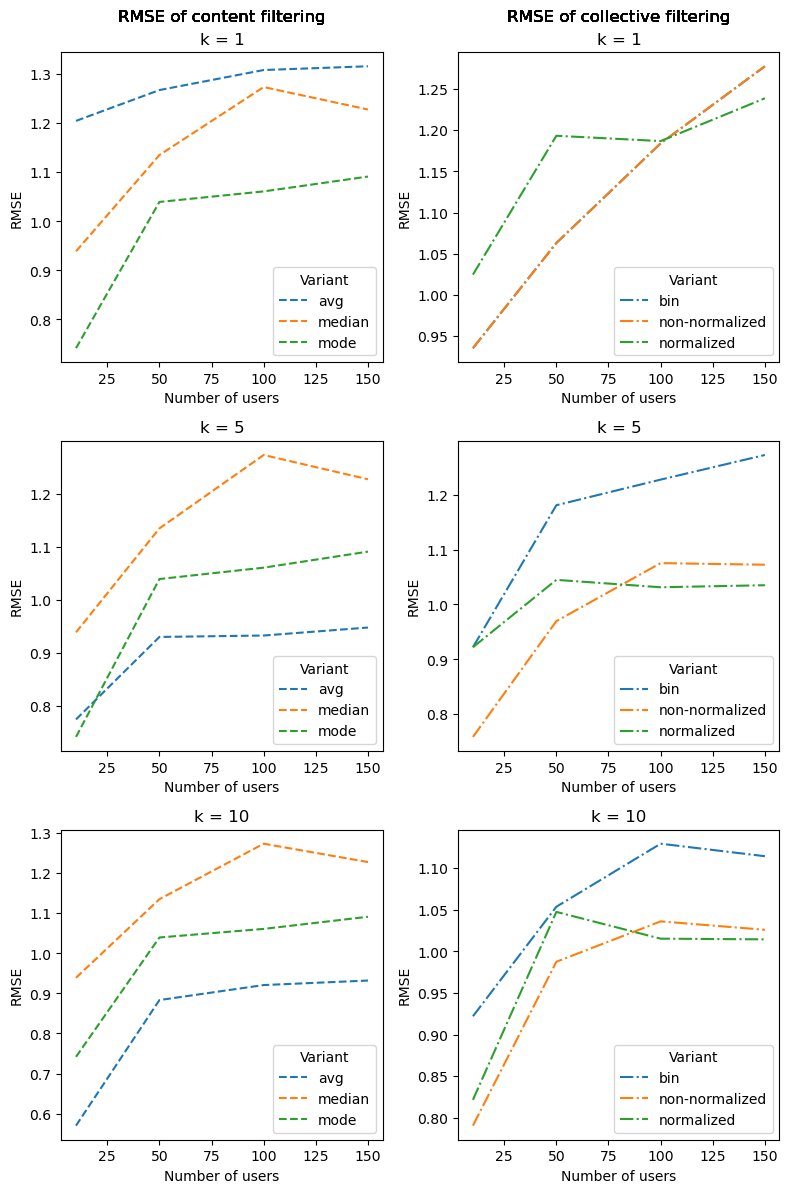
\includegraphics[width=0.9\textwidth]{figures/rmse-plot.png} 
    \caption{RMSE of 2 methods with different parameters}
    \label{fig:rmseplot}
\end{figure}

\autoref{fig:rmseplot} shows the RMSE of each method with variants and different parameters. 

\section{Conclusion}

In conclusion, in general we see that content-based is an simple but effective method for movie recommendation system, with fast calculation time and relatively high accuracy rate. 

It is important to note that in this project, we did not employ any complex machine learning algorithms or train the model using data. Instead, we interacted solely with the Neo4j GraphDatabase. However, Neo4j also provides Graph Data Science, a powerful machine learning library that supports more sophisticated algorithms, such as Linear Regression, Logistic Classification, Gradient Descent, and others. There are also specific algorithm built for graph structures, such as Node Classification, Node Regression and Link Prediction \footnote{More information at Neo4j website: \href{https://neo4j.com/product/graph-data-science/}{https://neo4j.com/product/graph-data-science/}}. Although the implementation of these libraries is beyond the scope of our report, we believe that Graph Data Science is a rapidly growing field with significant potential.

% \bibliographystyle{alpha}
% \bibliography{sample}

\end{document}